\documentclass[conference]{IEEEtran}
\IEEEoverridecommandlockouts
% The preceding line is only needed to identify funding in the first footnote. If that is unneeded, please comment it out.
\usepackage{cite}
\usepackage{amsmath,amssymb,amsfonts}
\usepackage{algorithmic}
\usepackage{graphicx}
\usepackage{textcomp}
\usepackage{xcolor}
\def\BibTeX{{\rm B\kern-.05em{\sc i\kern-.025em b}\kern-.08em
    T\kern-.1667em\lower.7ex\hbox{E}\kern-.125emX}}
\begin{document}

\title{Conference Paper Title*\\
{\footnotesize \textsuperscript{*}Note: Sub-titles are not captured in Xplore and
should not be used}
\thanks{Identify applicable funding agency here. If none, delete this.}
}

\author{
\IEEEauthorblockN{1\textsuperscript{st} Karina Heins}
\IEEEauthorblockA{\textit{DHBW Ravensburg Campus Friedrichshafen} \\
\textit{Mercedes-Benz AG}\\
Friedrichshafen,  Germany \\
heins.karina-tfe18@it.dhbw-ravensburg.de}
\and
\IEEEauthorblockN{2\textsuperscript{st} Florian Schatz}
\IEEEauthorblockA{\textit{DHBW Ravensburg Campus Friedrichshafen} \\
\textit{Mercedes-Benz AG}\\
Friedrichshafen,  Germany \\
schatz.florian-tfe18@it.dhbw-ravensburg.de}
\and
\IEEEauthorblockN{3\textsuperscript{st} Patrick Madlindl}
\IEEEauthorblockA{\textit{DHBW Ravensburg Campus Friedrichshafen} \\
\textit{Mercedes-Benz AG}\\
Friedrichshafen,  Germany \\
madlindl.patri-tfe18@it.dhbw-ravensburg.de}
\and
\IEEEauthorblockN{4\textsuperscript{st} Marcel Dirschinger}
\IEEEauthorblockA{\textit{DHBW Ravensburg Campus Friedrichshafen} \\
\textit{Airbus Helicopters AG}\\
Friedrichshafen,  Germany \\
dirschinger.marcel-tfe18@it.dhbw-ravensburg.de}
}

\maketitle

\begin{abstract}
This document is a model and instructions for \LaTeX.
This and the IEEEtran.cls file define the components of your paper [title, text, heads, etc.]. *CRITICAL: Do Not Use Symbols, Special Characters, Footnotes, 
or Math in Paper Title or Abstract.
\end{abstract}

\begin{IEEEkeywords}
component, formatting, style, styling, insert
\end{IEEEkeywords}

\section{Einleitung}

\section{Grundlagen}

\subsection{Merge Sort}
 \subsection{Message Passing Interface}
 \subsection{Cloud Computing}
\section{Umsetzung}
\subsection{Test}
Für das Projekt werden parallel zur Entwicklung der Funktionen Unit Tests mitverfasst. Hierfür verwendet wird die Testsuite \textit{gtest}, welche in \textit{GoogleTest} enthalten ist. Der Zweck der Unit Tests beschränkt sich auf eine Absicherung der Lauffähigkeit und Gewährleistung der Grundfunktionalität des Programms.
\\
Einige Funktionen, welche komplexe Algorithmen enthalten, werden mithilfe von im Vorhinein definierten \textit{Blackbox-Tests} entwickelt. Beispiele sind die Funktionen \textit{split\_even()} und \textit{merge\_back()}. Es werden jeweils ein Standard-Fall und mehrere Randfälle aus verschiedenen Äquivalenzklassen in die Tests aufgenommen. 
Wenn die zu entwickelnden Funktionen diese Tests bestehen, wird angenommen, dass die geforderte Grundfunktionalität erfüllt wird. Robustheit ist nicht gegeben. Eine vollständige Testabdeckung,
wie z.B. die \textit{vollständige Anweisungsüberdeckung} (C0-Überdeckung), wird nicht realisiert.
\\
Auf eine vollständige Testabdeckung nach einer der bekannten Klassen C0...C3 für strukturelle Tests wird generell verzichtet. Gründe hierfür sind die beschränkte Bearbeitungszeit für das Projekt sowie dass eine vollständige Abdeckung nicht zielführend für das Projekt ist. Das Testen von Nutzereingaben im Programm oder der MPI-Funktionalität würde einen hohen Aufwand beim Testentwurf bedeuten. Um die MPI-Funktionalitäten rigoros zu testen, müssten u.a. der Einfluss der Anzahl verwendeter Rechenknoten, die Behandlung von Knoten-Ausfällen sowie die Auswirkungen maximaler Nachrichtenpaketgrößen betrachtet werden. Hiervon wird abgesehen, da die im Rahmen des Projekts entworfene Software nicht produktiv eingesetzt wird und ausschließlich der Übung mit sowie der Demonstration von Vor- und Nachteilen von MPI dient. Die Vorteile einer vollständigen Testabdeckung würden in keinem Verhältnis zum benötigten Aufwand der Testerstellung stehen.
\\
Wäre eine Absicherung der Software durch Tests gewünscht, müssten die eigens entwickelten und implementierten Algorithmen rigoroser getestet werden. Für die Funktionen \textit{split\_even()} und \textit{merge\_back()} wird eine \textit{Zweigüberdeckung} (C1) als sinnvoll betrachtet, da diese Funktionen eine zentrale Rolle in der Software einnehmen. Die Funktionalitäten des Merge Sort Algorithmus können weiterhin mit geringer Testabdeckung in Form von Blackbox Tests oder \textit{Anweisungsüberdeckung} (C0) für eine Rekursionsebene des Algorithmus gewährleistet werden.
Dies wird ist durch die allgemein bekannte Korrekheit des Algorithmus gerechtfertigt.
\subsection{Parallelisierung}
\section{Ergebnis}
\subsection{Optimierung}
Grundsätzlich versprechen sich die Autoren von richtig implementierter Parallelisierung einen messbaren Zusammenhang von der Anzahl der verwendeten Rechenknoten und der resultierenden Laufzeit.
Um diese These zu überprüfen, und weitere mögliche Zusammenhänge zu erfassen, wurden im Rahmen der Arbeit umfassende Laufzeitmessungen durchgeführt.
Um Vergleichbarkeit herzustellen, wurden alle Messungen innerhalb kürzester Zeit am gleichen Tag vorgenommen. Aufgrund beschränkter Zeit wurde eine Stichprobengröße von $n = 10$ Messungen pro Messklasse gewählt.
Es sei angemerkt: wünschenswert und für eine statistisch fundierter Aussage notwendig wäre das fünf bis zehnfache hiervon. \paragraph
Die Messklassen werden hier über die Anzahl der verwendeten Rechenknoten festgelegt; für die Auswertung wurden Messungen mit einem bis sieben Rechenknoten durchgeführt.
Gemessen wird jeweils die benötigte Laufzeit, eine wohldefinierte und unveränderliche Datei bestehend aus einer großen Zahl von Wörtern zu sortieren.
Eine Messergebnis ist die mithilfe der Standard Template Bibliothek std::chrono gemessene Zeit, welche im Programmablauf des Master-Knotens zwischen dem Zeitpunkt unmittelbar vor der Verteilung der Teilelemente 
des zu sortierenden Textes an die Slave-Knoten und dem Zeitpunkt unmittelbar nach dem Zusammenführen der Ergebnisse der Slave-Rechenknoten verstreicht.
Das arithmetische Mittel sowie die Standardabweichung der Messreihen sind in Tabelle 1 aufgeführt.

\begin{table}
    \centering
    \caption{Zeitmessungen mit verschiedenen Anzahlen an Rechenknoten}
    \label{zeiten_tabelle}
    \begin{tabular}{l|lllllll}
    \textbf{Anzahl der Rechenknoten}  & \textbf{1} & \textbf{2} & \textbf{3} & \textbf{4} & \textbf{5} & \textbf{6} & \textbf{7}  \\ 
    \hline\hline
    \%\textbackslash{}bar\{t\}\$ [ms] & 4382.9     & 2413.7     & 2148.5     & 1728.6     & 1715.9     & 1621.6     & 1574.6      \\
    \$\textbackslash{}sigma\$ [ms]    & 491.2      & 128.0      & 113.9      & 72.2       & 70.9       & 62.3       & 112.4      
    \end{tabular}
\end{table}

Bei der Messreihe mit genau einem Rechenknoten ist eine erhöhte Unsicherheit zu erkennen. Dennoch ist der Mittelwert signifikant höher als bei allen anderen 
Messungen mit einer Rechenknotenanzahl größer eins. Bei den Anzahlen vier, fünf und sechs ist eine im Vergleich geringe Abweichung festzustellen. Diese Werte haben eine entsprechend hohe 
Aussagekraft. Interessanterweise sind die Mittelwerte der Zeiten ab einer Rechenknotenanzahl von 4 sehr nah beieinander. Daher kann mit den vorliegenden Daten keine statistisch begründete Aussage getroffen werden, ob sich die Rechenzeit ab einer Knotenzahl von 4 noch messbar verändert. Hierfür liegen die Messungen zu nah beieinander. Der scheinbar deutlich niedrigere Mittelwert der 7. Messung wird durch eine
höhere Messunsicherheit relativiert.

\paragraph

Eine umfassendere Darstellung der Daten erfolgt mithilfe eines Whiskers Plots, auch Kastenschaubild genannt (Abbildung X). Auch hier ist die vermutete, anfängliche und deutliche 
Absenkung der Laufzeiten über die Anzahl der Rechenknoten zu erkennen. Ebenfalls fällt ein starker Ausreißer bei der Knotenzahl eins auf. Auch bei Knotenzahlen zwei, vier und sechs 
gibt es solche Ausreißer. Interessanterweise gibt es gerade bei den Knotenzahlen vier und sechs, welche eine relativ geringe Standardabweichung aufweisen, ebenfalls Ausreißer nach oben. 
Im Kontext der niedrigen Standardabweichung bedeutet das einerseits, dass die restlichen Messwerte dieser Messreihen besonders konsistent sind. Andererseits könnte dies ein Hinweis darauf sein, dass die gemessenen Zeiten durch Zufall besonders konsistent und niedrig ausgefallen sind.

\begin{figure}[!t]
    \centering
    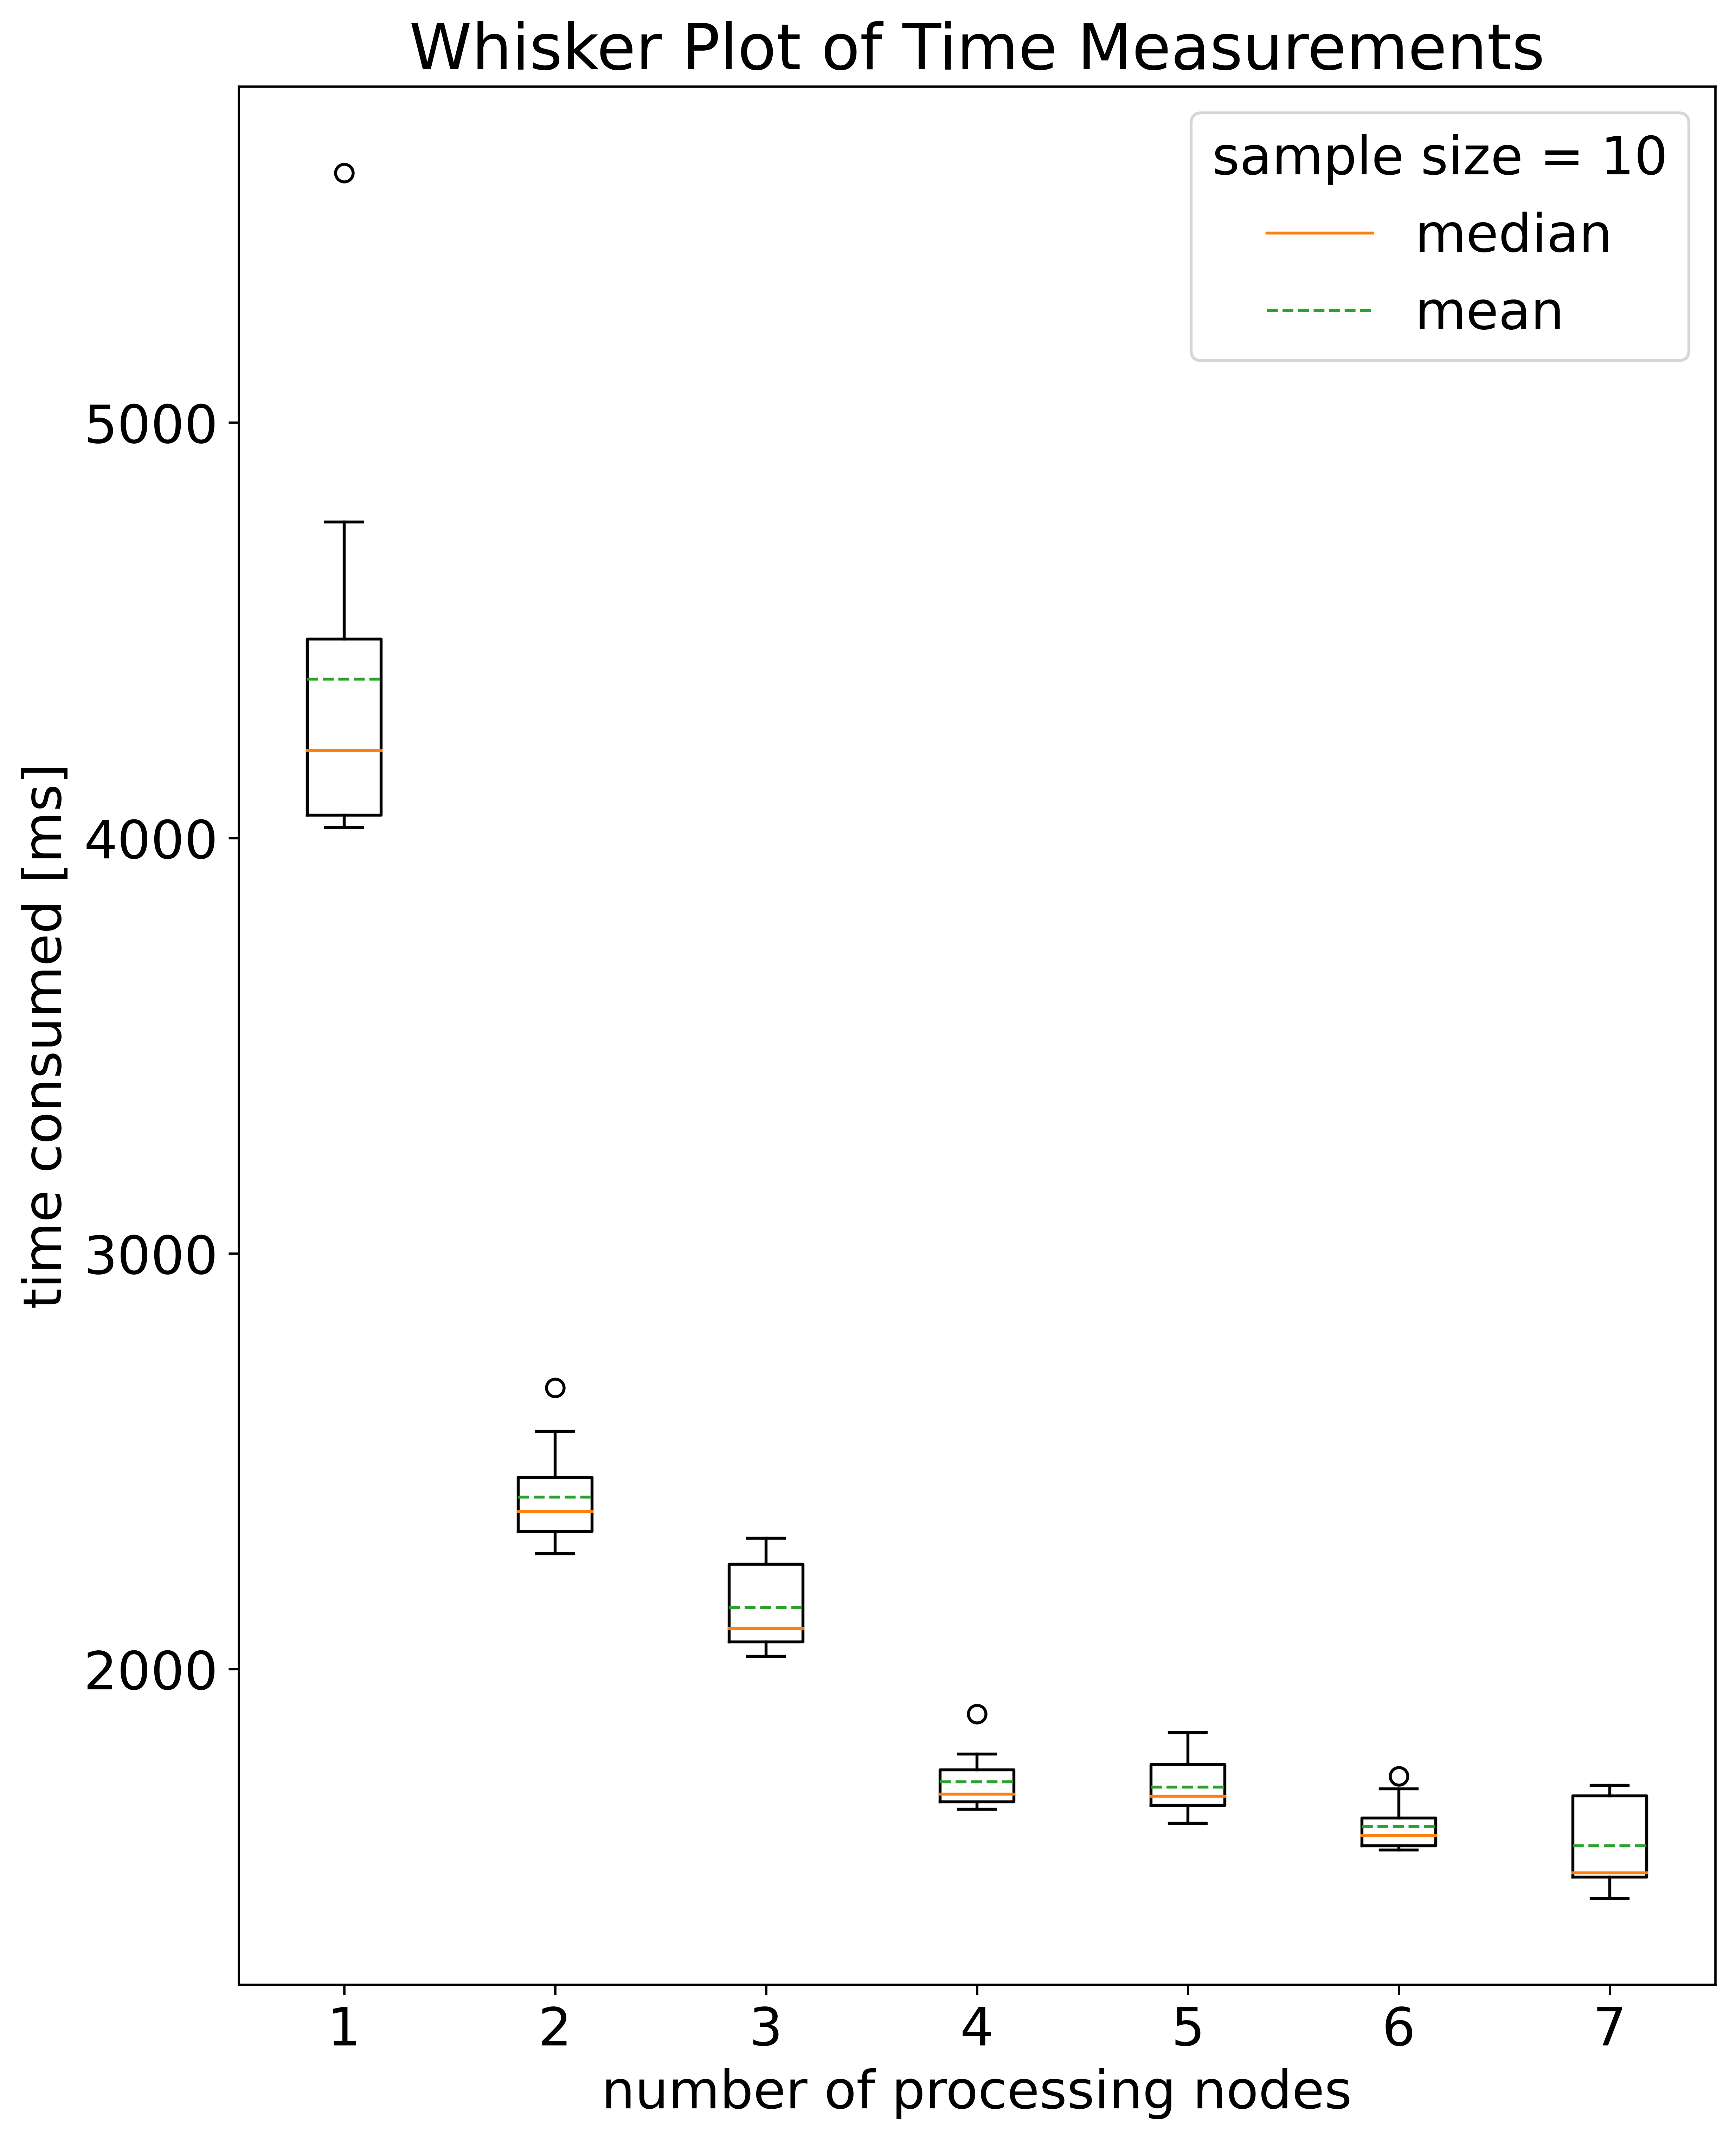
\includegraphics[width=8in]{boxplots.png}
    \caption{Cpation is already in picture!}
    \label{boxplot_times}
\end{figure}

\paragraph

So lassen die beobachteten Phänomene insgesamt darauf schließen, dass die Parallelisierung in ihrer für das Projekt durchgeführten Implementierung eine signifikante Absenkung der Laufzeit von bis zu einer Größenordnung von 60\% mit sich bringt. Dieser Effekt ist jedoch stark begrenzt und flacht mit einer steigenden Rechenknotenanzahl schnell ab bzw. verschwindet gänzlich. Die Effizienz pro Rechenknoten nimmt damit bei steigender Anzahl von Rechenknoten schnell ab.
Für genauere Aussagen ist eine größere Anzahl an Messungen pro Messklasse für nötig.

\paragraph

Eine Deutung für die Beobachteten Ergebnisse: die Rechenknoten in der Cloud sind mittels Ethernet miteinander verbunden, was das Senden und Empfangen von Nachrichten erstens nicht zeitlich deterministisch und zweitens anfällig für unregelmäßige und längere Laufzeiten macht. Offenbar bewegt sich bei der betrachteten Dateigröße das Senden und Empfangen von Nachrichten an mehr Knoten ab einer Knotenzahl von ca. vier in einer ähnlichen Größenordnungen wie der Laufzeitgewinn, welcher dadurch entsteht, dass ein Rechenknoten nur eine geringere Anzahl an Arbeit (Wörter sortieren) hat. Die Autoren vermuten, dass bei einer deutlich größeren Datei (mit mehr Wörtern), ein Laufzeitgewinn auch bei größeren Knotenzahlen zu messen sein wird.

\section{Fazit}

\section*{Acknowledgment}

The preferred spelling of the word ``acknowledgment'' in America is without 
an ``e'' after the ``g''. Avoid the stilted expression ``one of us (R. B. 
G.) thanks $\ldots$''. Instead, try ``R. B. G. thanks$\ldots$''. Put sponsor 
acknowledgments in the unnumbered footnote on the first page.

\section*{References}

Please number citations consecutively within brackets \cite{b1}. The 
sentence punctuation follows the bracket \cite{b2}. Refer simply to the reference 
number, as in \cite{b3}---do not use ``Ref. \cite{b3}'' or ``reference \cite{b3}'' except at 
the beginning of a sentence: ``Reference \cite{b3} was the first $\ldots$''

Number footnotes separately in superscripts. Place the actual footnote at 
the bottom of the column in which it was cited. Do not put footnotes in the 
abstract or reference list. Use letters for table footnotes.

Unless there are six authors or more give all authors' names; do not use 
``et al.''. Papers that have not been published, even if they have been 
submitted for publication, should be cited as ``unpublished'' \cite{b4}. Papers 
that have been accepted for publication should be cited as ``in press'' \cite{b5}. 
Capitalize only the first word in a paper title, except for proper nouns and 
element symbols.

For papers published in translation journals, please give the English 
citation first, followed by the original foreign-language citation \cite{b6}.

\begin{thebibliography}{00}
\bibitem{b1} G. Eason, B. Noble, and I. N. Sneddon, ``On certain integrals of Lipschitz-Hankel type involving products of Bessel functions,'' Phil. Trans. Roy. Soc. London, vol. A247, pp. 529--551, April 1955.
\bibitem{b2} J. Clerk Maxwell, A Treatise on Electricity and Magnetism, 3rd ed., vol. 2. Oxford: Clarendon, 1892, pp.68--73.
\bibitem{b3} I. S. Jacobs and C. P. Bean, ``Fine particles, thin films and exchange anisotropy,'' in Magnetism, vol. III, G. T. Rado and H. Suhl, Eds. New York: Academic, 1963, pp. 271--350.
\bibitem{b4} K. Elissa, ``Title of paper if known,'' unpublished.
\bibitem{b5} R. Nicole, ``Title of paper with only first word capitalized,'' J. Name Stand. Abbrev., in press.
\bibitem{b6} Y. Yorozu, M. Hirano, K. Oka, and Y. Tagawa, ``Electron spectroscopy studies on magneto-optical media and plastic substrate interface,'' IEEE Transl. J. Magn. Japan, vol. 2, pp. 740--741, August 1987 [Digests 9th Annual Conf. Magnetics Japan, p. 301, 1982].
\bibitem{b7} M. Young, The Technical Writer's Handbook. Mill Valley, CA: University Science, 1989.
\end{thebibliography}
\vspace{12pt}
\color{red}
IEEE conference templates contain guidance text for composing and formatting conference papers. Please ensure that all template text is removed from your conference paper prior to submission to the conference. Failure to remove the template text from your paper may result in your paper not being published.

\end{document}
